 A Figura~\ref{fig:architecture} ilustra a arquitetura completa. A cada instante de decisão, o módulo \acrotip{TOPSIS} processa as informações multicritério sobre todos os candidatos viáveis e produz o vetor de estado 6D que é passado ao agente \acrotip{SAC}.

\begin{figure}[t]
  \centering
  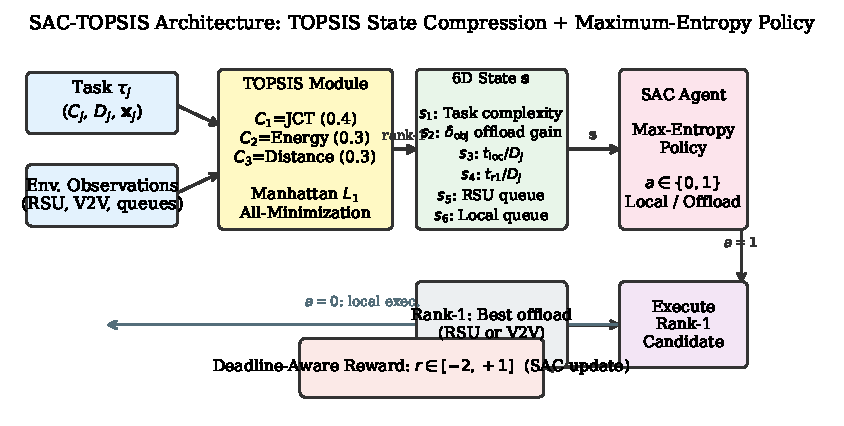
\includegraphics[width=\columnwidth]{images/fig_01_architecture.pdf}
  \caption{Arquitetura \acrotip{SAC}-\acrotip{TOPSIS}.
           O \acrotip{TOPSIS} comprime o conjunto de candidatos de tamanho variável em um
           vetor de estado fixo 6D invariante à escala.
           O \acrotip{SAC} aprende uma política binária (local vs.\ melhor descarregamento)
           sobre essa representação com regularização de máxima entropia.}
  \label{fig:architecture}
\end{figure}

\subsection{Compressão de Estado Baseada em \acrotip{TOPSIS}}
\label{sec:topsis}

\paragraph{Matriz de decisão.}
Para a tarefa $\tau_j$, construímos uma matriz de decisão
$\mathbf{X} \in \mathbb{R}_{\ge 0}^{3\times 3}$ cujas linhas correspondem aos
três modos candidatos (local, \acrotip{RSU}, \acrotip{V2V}) e cujas colunas são os três critérios
de custo:
\begin{equation}
  \mathbf{X} =
  \begin{bmatrix}
    \mathrm{JCT}_j^{(0)} & E_j^{(0)} & 0 \\
    \mathrm{JCT}_j^{(1)} & E_j^{(1)} & d_{\mathrm{RSU}} \\
    \mathrm{JCT}_j^{(2)} & E_j^{(2)} & d_{\mathrm{V2V}}
  \end{bmatrix},
  \label{eq:dm}
\end{equation}
onde $d_{\mathrm{RSU}}$ e $d_{\mathrm{V2V}}$ são as distâncias euclidianas
ao \acrotip{RSU} e ao par \acrotip{V2V} selecionado, respectivamente.
Se um modo for inviável, sua linha é definida como $10^6$ para excluí-lo das
soluções ideais.

\paragraph{Normalização ponderada.} Cada coluna $j$ é normalizada por sua norma euclidiana $\|\mathbf{X}_{:j}\|_2$ e depois multiplicada pelo peso $w_j \in \{0{,}4;\, 0{,}3;\, 0{,}3\}$ (\acrotip{JCT}, energia, distância), resultando na matriz normalizada ponderada $\widetilde{\mathbf{X}}$.

\paragraph{\acrotip{TOPSIS} $L_1$-Manhattan.}
Diferimos do \acrotip{TOPSIS} clássico medindo distâncias à solução ideal positiva (\acrotip{PIS})
$A^+$ e à solução ideal negativa (\acrotip{NIS}) $A^-$ usando a norma Manhattan
($L_1$):
\begin{equation}
  D_i^+ = \textstyle\sum_{k} \lvert \widetilde{x}_{ik} - A_k^+ \rvert,
  \qquad
  D_i^- = \textstyle\sum_{k} \lvert \widetilde{x}_{ik} - A_k^- \rvert.
  \label{eq:manhattan}
\end{equation}
O escore de proximidade é então $\mathcal{C}_i = D_i^- / (D_i^+ + D_i^-)$.
Como todos os critérios são objetivos de minimização de custo, $A^+$ é o
mínimo coluna a coluna e $A^-$ é o máximo coluna a coluna de
$\widetilde{\mathbf{X}}$.
A métrica $L_1$ é menos sensível a valores extremos, propriedade crítica quando
as estimativas de fila são ruidosas, e é computacionalmente mais leve que $L_2$.

\paragraph{Seleção do rank-1.}
O candidato de descarregamento rank-1 é o modo não local viável com o
maior $\mathcal{C}_i$:
\begin{equation}
  m^* = \operatorname*{argmax}_{i \in \{1,2\}} \mathcal{C}_i
        \;\text{s.t.\ modo } i \text{ é viável}.
  \label{eq:rank1}
\end{equation}
Empates são resolvidos em favor do \acrotip{V2V} para estimular balanceamento de carga.
Se nenhum modo de descarregamento for viável, $m^*$ recorre à execução local
independentemente da ação do agente.

\paragraph{Vetor de estado 6D.}
O estado $\mathbf{s} \in \mathbb{R}^6$ é montado como:
\begin{align}
  s_1 &= C_j / 10^{10} \notag \\
  s_2 &= \mathrm{clip}\!\left(1 - \frac{\mathrm{custo}_{m^*}}{\mathrm{custo}_{\mathrm{loc}}},\,-1,1\right) \notag \\
  s_3 &= \min\!\left(1,\; \mathrm{\acrotip{JCT}}^{(0)} / D_j\right) \notag \\
  s_4 &= \min\!\left(1,\; \mathrm{\acrotip{JCT}}^{(m^*)} / D_j\right) \notag \\
  s_5 &= \min\!\left(1,\; |Q_{\mathrm{\acrotip{RSU}}}| / 25\right) \notag \\
  s_6 &= \min\!\left(1,\; |Q_{v_0}| / 25\right)
  \label{eq:state}
\end{align}
{\scriptsize onde os componentes representam: complexidade da tarefa; vantagem do descarregamento; urgência local; urgência rank-1; ocupação da fila \acrotip{RSU}; e ocupação da fila local.}
onde $\mathrm{custo}_m = \alpha\,\mathrm{JCT}^{(m)} + \beta\,E^{(m)}$.
Todos os componentes pertencem a $[0,1]$ ou $[-1,1]$, tornando $\mathbf{s}$
invariante à escala, pois não depende do número de candidatos disponíveis,
apenas da qualidade relativa do melhor deles.

\subsection{Soft Actor-Critic de Máxima Entropia}
\label{sec:sac}

O agente \acrotip{SAC} otimiza o objetivo de máxima entropia~\cite{haarnoja2018sac}:
\begin{equation}
  \pi^* = \operatorname*{argmax}_\pi\;
  \mathbb{E}_{\tau \sim \pi}\!\left[
    \sum_{t} \gamma^t \bigl(r_t + \alpha_T\,\mathcal{H}[\pi(\cdot\mid s_t)]\bigr)
  \right],
  \label{eq:sac_obj}
\end{equation}
onde $\alpha_T$ é o parâmetro de temperatura ajustado automaticamente.
As redes ator e crítico são MLPs com duas camadas ocultas de 256~unidades e
ativações ReLU.
O ator gera logits para a distribuição de ação de Bernoulli; a temperatura
$\alpha_T$ é adaptada para uma entropia alvo de $\log 2 / 2$ nats.
O buffer de replay armazena $10^5$ transições; o tamanho do mini-lote é $256$;
a taxa de aprendizado é $3 \times 10^{-4}$ para todas as redes.

\paragraph{Por que ação binária?} Delegar a seleção do destino de descarregamento ao \acrotip{TOPSIS} reduz o espaço de ações de $|\mathcal{V}(t)| + 2$ dimensões a um único bit. Essa simplificação é sem perda da perspectiva do agente, pois a ordenação relativa dos candidatos já está codificada em $s_2$--$s_4$.

\subsection{Função de Recompensa Ciente do Prazo}
\label{sec:reward}

A recompensa $r_j$ para a tarefa $\tau_j$ é projetada para guiar o agente ao
cumprimento do prazo enquanto fornece um sinal de gradiente contínuo:
\begin{equation}
  r_j = \begin{cases}
    1{,}0 - 0{,}5 \cdot \rho_j        & \text{se } \mathrm{JCT}_j \le D_j, \\
    -1{,}0 - \min(1,\,\delta_j)       & \text{caso contrário,}
  \end{cases}
  \label{eq:reward}
\end{equation}
onde
\begin{equation}
  \rho_j = \tfrac{1}{2}\!\left(\frac{\mathrm{JCT}_j}{D_j}
                              + \frac{E_j}{E_{\max,j}}\right) \in [0,1]
  \label{eq:rho}
\end{equation}
é uma razão de custo normalizada, e $\delta_j = (\mathrm{JCT}_j - D_j)/D_j$
é a violação relativa do prazo.
Execuções bem-sucedidas rendem $r_j \in [0{,}5,\,1{,}0]$: tarefas mais rápidas
e eficientes recebem recompensas maiores.
Execuções com falha rendem $r_j \in [-2,\,-1]$: a penalidade cresce com o
grau de atraso, fornecendo um gradiente que ensina o agente a
falhar pelo menor tempo possível.
